\documentclass{tikzposter}
\usepackage{graphicx}
\usepackage{float}
\title{Interactive Simulations for CfE Physics}
\author{Craig Roy\vspace{0.5cm}\\Supervisor: Gordon Robb\vspace{0.4cm}}
\institute{University of Strathclyde}
\definecolor{strathBlue}{RGB}{2,30,73}
\definecolor{strathGreen}{RGB}{88,136,24}
\definecolorpalette{myColours} {
  \colorlet{colorOne}{white}
  \colorlet{colorThree}{yellow}
  \colorlet{colorTwo}{strathGreen}}
\usebackgroundstyle{Default}
\usecolorstyle[colorPalette=myColours]{Default}
\usetitlestyle{Wave}
\useblockstyle{Basic}
\usenotestyle{Sticky}
\begin{document}
\maketitle
  \begin{columns}
    \column{0.5}
    \block{The Project}{
      \paragraph{Aim}
      The aim of this project was to create interactive simulations to aid the teaching of the new Higher and Advanced Higher Physics Curriculum for Excellence courses.
      \paragraph{Motivation}
      Since the Curriculum for Excellence programme was implemented, there has been a demand for resources to aid in teaching the new elements of the Higher and Advanced Higher Physics curriculum.
      \paragraph{Topics}
The topics chosen for this project were: Special Relativity, Particle Accelerators and The Doppler Effect.
These topics were all introduced with the Curriculum for excellence
program. The topics were chosen for this project from a
SUPA video competition with the same goal of creating more
resources for the new physics courses.
    }
    \block{Practical Considerations}{
    The tool used to create the simulations was a program called EjsS or
``Easy Java(Script) Simulations''. EjsS is a tool created as a part of the Open Source Physics project. It is designed to make creating computer simulations easy for people such as science teachers and students who are otherwise unfamiliar with programming in Java or JavaScript.

This program was chosen so that simulations could be developed with
relative ease, and so that there is a no barrier to entry for someone
who wants to modify the simulations. Developing the simulations as
Java programs also meets the needs of physics teachers who cannot
access the internet while teaching to view Flash simulations or Java Applets.
}
    \block{Special Relativity I}{The first simulation shows a pair of digital clocks. One relatively stationary in a lab, and the other travelling at a relativistic speed specified by the user. The observer is in the reference frame of the lab clock and can observe the slowing down of the moving clock.
      \begin{tikzfigure}
    \includegraphics[width=0.8\linewidth]{./images/digitalUI.png}
    \end{tikzfigure}}
    \block{Special Relativity II}{The second simulation shows a pair of analogue clocks, one of which is travelling at relativistic speeds. In this experiment, the observer is in the reference frame of the clock travelling at a relativistic speed specified by the user. The user can observe that the stationary clock speeds up as the velocity is increased.
\begin{tikzfigure}
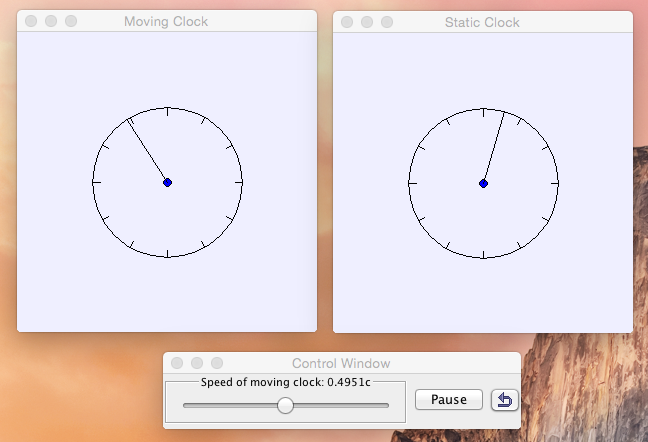
\includegraphics[width=0.8\linewidth]{./images/analogueUI.png}
\end{tikzfigure}}
    \column{0.5}
    \block{Special Relativity III}{This experiment shows a pair of model photon clocks, with a 'photon' bouncing between two mirrors. The user is in the reference frame of the lab clock.

As the user sets the speed of the moving clock, it begins to move across the window. At relativistic speeds, the motion of the photon appears to slow and the moving photon clock contracts in size due to time dilation.

\begin{tikzfigure}
  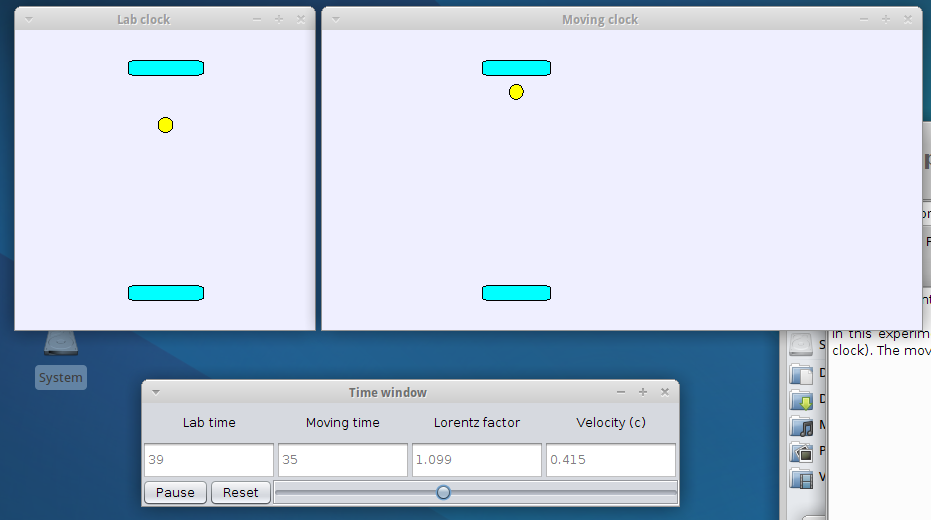
\includegraphics[width=0.8\linewidth]{./images/mirrorUI.png}
\end{tikzfigure}}

    \block{Cyclotron}{This experiment models a cyclotron particle accelerator which is relevant to the electromagnetism section of the Advanced Higher course. The user may set variables such as the strength of the electric field, the charge of the particle, and the frequency of oscillation of the electric field and the accelerator will apply the Lorentz force accordingly.
\begin{tikzfigure}
  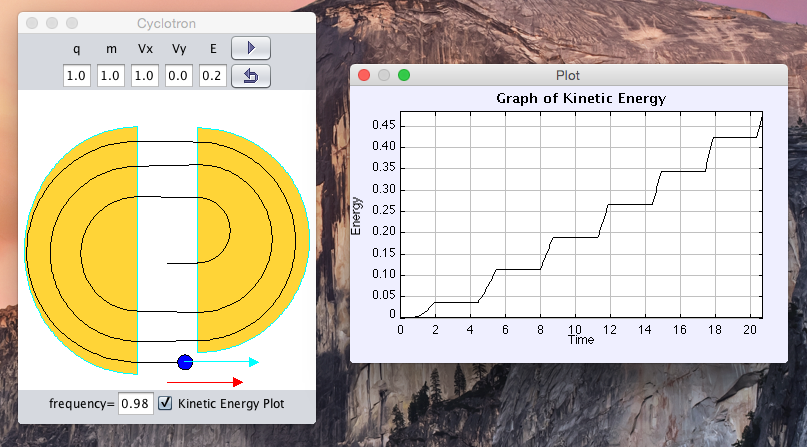
\includegraphics{./images/cycloUI.png}
    \end{tikzfigure}}
    \block{Doppler Effect}{This simulation demonstrates the concept of the doppler shift as well as the concept of using spectroscopy on exoplanets.

The simulation consists of a model exoplanet which is orbiting a star. The planet is being monitored using spectroscopy. The absorption lines are shown on a spectrum of visible light at the bottom of the window.

The user chooses the angular velocity of the planet and star, and a Doppler shift is applied to the spectral lines when the planet is moving towards the observer or further away.
\begin{tikzfigure}
  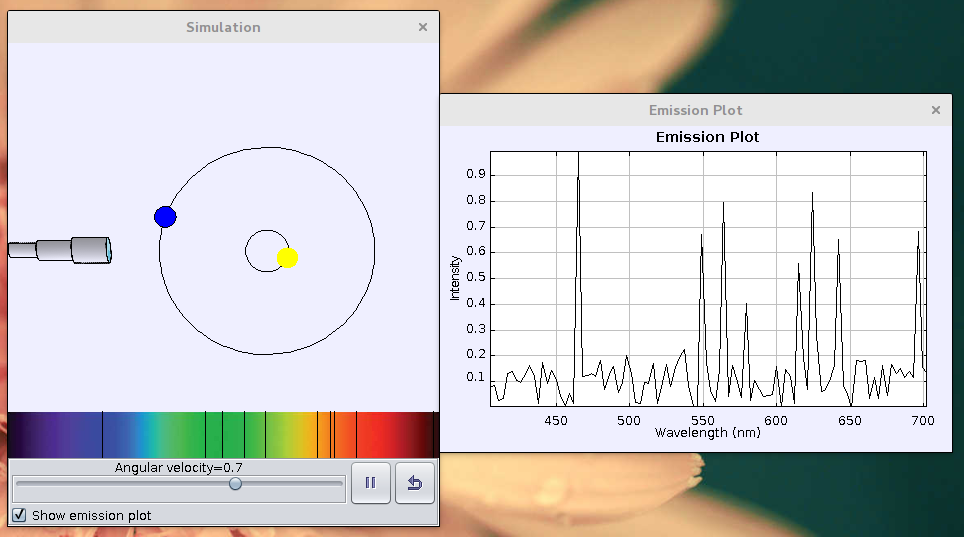
\includegraphics{./images/dopplerUI.png}
    \end{tikzfigure}}
  \end{columns}
\end{document}
